\label{sec:stats}
Once the experiment has been conducted and the data has been recorded, 
physicists might be interested in asking questions such as,
did one or did one not establish a discovery? Or,
how well does an alternate model describe this discovery?
The first question has to do with the goodness of the fit of the 
observed data to the good and old Standard Model,
while the second question has to do with hypotheses testing and the derivation of 
confidence intervals and upper limits~\cite{Stats-for-pedestrian}.
In order to answer these questions, one needs to first define the null hypothesis $H_0$ and
the alternative hypothesis $H_1$.
The definition of $H_1$ and $H_0$ depends of the specific physics problem, using the tone
of the particle physics, for search for a new signal process, the null hypothesis $H_0$ is 
assuming only the background is observed, the alternative hypothesis $H_1$ is assuming 
one observes both signal and background; for problems such as setting upper limits,
this definition is reversed.

It is common to refer to the \textit{p-value} to quantity the deviation from the null hypothesis, 
which is defined as:
\[
p = \int_{x_{obs}}^\infty g(x|H_0) dx,
\addtag \]
where $g(x|H_0)$ is the probability density function of observing a quantity
$x$ given the null hypothesis, and $x_{obs}$ is the observed value. The p-value derivation 
is shown illutratively in Figure~\ref{fig:stats:pvalue}, together with $\alpha$, 
which is defined as:
\[
\alpha = \int_{x_{5\sigma}}^\infty g(x|H_0) dx,  
\addtag \]
where $x_{5\sigma}$ is the observed value that corresponds $5\sigma$ deviation 
from the null hypothesis. 
One can therefore claim a discovery if the observed p-value $p < \alpha$ (equivalently, 
the background-only null hypothesis is rejected with a probability $1-p$).
Another commonly used statistic jargon is the \textit{confidence level} ($CL$),
which is defined as:
\[
CL   = \int_{ -\infty}^{x_{5\sigma}} g(x|H_0) dx \equiv 1- p .
\addtag \]
Lastly, the p-value is oftenly converted to a significance $Z$, 
defined as the number of standard deviations above the mean of a Gaussian distribution.
The relation between the p-value and $Z$ is given by:
\[
Z=\Phi^{-1} (1-p),
\addtag \]
where $\Phi^{-1}$ is the quantile function of the standard Gaussian distribution.
The discovery of signal, as mentioned before, needs to be rejecting the background-only hypothesis
with at least $Z \ge 5$, which corresponds to a p-value of $2.87 \times 10^{-7}$.
In the case of setting upper limits, for excluding the signal hypothesis, p-value is by convention 
required be less than 0.05 (95\% confidence level), which is equivalent to $Z = 1.64$.
This value is also used for setting upper limits in chapter~\ref{sec:search for dihiggs}.
N.B.\ In chapter~\ref{sec:search for dihiggs}, 
the $CL$ used for setting upper limits is calculated by the $CL_s$ method~\cite{CLs}
where $CL_s$ is (unfortunately named $CL_s$) given by:
\[
    CL_s   =  \frac{p_{s+b}}{1-p_b},
\addtag \]
where $p_{s+b}$ and $p_b$ are the confidence leveles for the signal-plus-background hypothesis
and the background-only hypothesis, respectively. 
The reason for using the $CL_s$ instead of the $p_{s+b}$ is that, in case of an experiment 
with low sensitivity, $1-p_b$ becomes small, and hence the signal will not 
be excluded even with a small p-value. 

\begin{figure}[htbp]
    \centering
    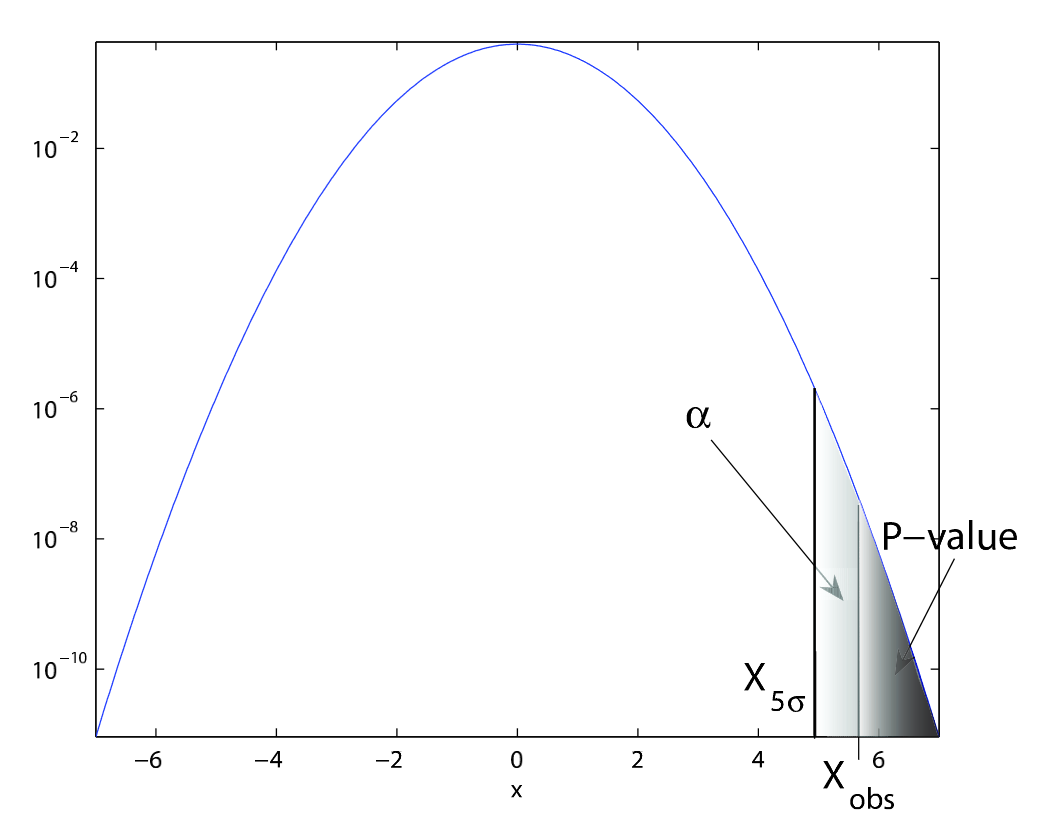
\includegraphics[width=0.6\textwidth]{theory/plots/pvalue.png}
    \caption{An illustration showing the control area $\alpha$ and the p-value of a Gaussian distribution. Note, in this 
    example $X_{obs} > X_{5\sigma}$. Image taken from Ref.\cite{Stats-for-pedestrian}}.
    \label{fig:stats:pvalue}
\end{figure}









\subsection{Test statistics}
A \textit{test statistic} is a quantity calculated from data,
which can be used to estimate how probable is the result 
that we observe with respect to some null hypothesis.
In terms of hypothesis testing, the observable $x$ is usually replaced by 
a test statistic $t$, so that the p-value becomes
\[
p = \int_{t_{obs}}^\infty g(t|H_0) dt.
\addtag \]
Due to the Neyman-Pearson lemma~\cite{Neyman-Pearson}, the most powerful test statistic
one can construct is given by:
\[
t  = \frac{L(H_1)}{L(H_0)},
\addtag \]
where $L(H_1)$ and $L(H_0)$ are the likelihood fuction of the hypothesis $H_1$ and $H_0$, respectively.
The analsysis discussed in this thesis in most of the time involves
signal and background, distributed in some histograms $\mathbf{n}$ of $N$ bins:
$\mathbf{n}  = (n_1, n_2, ... , n_N)$. In such case, 
the expectation of each bin is consists of the background $b$ and the signal $s$ with some signal
strength $\mu$:
\[
    E[n_i] = \mu s_i + b_i.
\addtag \]
In addition to the signal strength, it is common that the signal and background will depend
on some additional parameters, as referred to \textit{nuisance parameters}, that is
not of direct insterst of the analysis but needs to be fitted from the data. 
Hence, the expected signal and background is determined by the 
total signal and background and the respective probability function $f$ and 
nuisance parameters $\theta$~\cite{Glen-Cowan}:
\[
s_i = s_{tot} \int_i f_s(x;\mathbf{\theta}_s ) dx,
\addtag \]
\[
b_i = b_{tot} \int_i f_b(x;\mathbf{\theta}_b ) dx.
\addtag \]
In addition, these nuisance parameters are oftenly constrained by additional subsidiary measurements.
Suppose the measurements are distributed in a new histogram $\mathbf{m} = (m_1, ..., m_M)$,
and the expectation values of bin $m_i$ is given by $E[m_i] = u_i(\mathbf{\theta})$.

Since in a counting experiment, the data follows a Poisson distribution, 
the likelihood function can be written as:
\[
L(\mu, \mathbf{\theta}) = \prod^N_{j=1}    \frac{(\mu s_j + b_j )^{n_j}}{n_j !} e^{-(\mu s_j + b_j)}
\prod^N_{k=1} \frac{u_k^{m_k}}{m_k!}e^{-u_k} .
\addtag \]
One can define a profile likelihood ratio, such that:
\[
\lambda (\mu)  = \frac{L(\mu, \hat{\hat{\mathbf{\theta}}})}{L(\hat{\mu}, \hat{\mathbf{\theta}})},
\addtag \]
where $\hat{\mathbf{\theta}}$ and $\hat{\mu}$ are the maximum likelihood estimators,
that
\[
( \hat{\mathbf{\mu}}, \hat{\mathbf{\theta}} ) = argmax\ L(\mu, \theta).
\addtag \]
and $\hat{\hat{\mathbf{\theta}}}$ is the $\mathbf{\theta}$ that maximise $L$
for the specific $\mu$. 
As a result, the profile likelihood ratio has value $0 \le \lambda \le 1$, and for $\lambda$ value
close to 1, the hypothesis is well compatibile with the observed data. 

Using the profile likelihood ratio, one can define the test statistic as:
\[
t_\mu = -2 ln \lambda(\mu) ,
\addtag \]
and therefore, $t_\mu$ approaches to 0 from the positive direction, and corresponds to
a large p-value.  
For establishing a discovery of a positive signal, one can assume the signal 
strength $\mu \ge 0$. If data fluctuates below the expected  background, 
i.e.~$\hat{\mu} < 0$, it may constitute evidence against the background-only model, 
but this does not show that the data contain signal events
and the most physical explaination is that this is due to
some systematic error. Therefore, for \textbf{signal discovery},
the test statistic of the background-only null hypothesis  given by:
\[
  t_0 =q_0 =   \begin{cases}    
        -2 ln \lambda(0) \quad \hat{\mu} \ge 0, \\
        0  \qquad \qquad             \     \hat{\mu} < 0.
    \end{cases} 
\addtag \]

Consider the opposite case, for \textbf{setting upper limits} on a signal, one needs the test
statistic for the signal-plus-background null hypothesis with signal strength $\mu$, 
and if data fluctuates above signal plus background, i.e.~$\hat{\mu} > \mu$, 
the signal is not likely to be excluded and most likely is due to systematic errors. 
Therefore:
\[
  t_\mu =q_\mu =   \begin{cases}
    -2 ln \lambda(\mu) \quad \hat{\mu} \le \mu, \\
    0  \qquad \qquad  \   \             \hat{\mu} > \mu.
    \end{cases} 
\addtag \]



\subsection{Look elsewhere effect}
\label{sec:stats:look-elsewhere}
Suppose one specify an hypothesis with a specific Higgs mass and observed some signal at some mass range, 
one should also take into account that this signal could be a fluctuation which could be observed anywhere in
the sensitivity range~\cite{look-elsewhere}. This effect is referred to as \textit{look-elsewhere effect}.
A common belief is that the such effect is the reason for the
habit of defining a discovery as a 5~$\sigma$ and not for example 4~$\sigma$, 
because even if one quote 5~$\sigma$ the effective significance might be lower.
In this thesis, the look-elsewhere effect is accounted by calculating the global significance
following Ref.\cite{global-significance}, using the up-crossing method:
\[ p_\text{global} = p_\text{local} +  N_\text{up} e^{-1/2(Z^2_\text{local} - Z^2_\text{ref})},
\addtag \]
where the $p_\text{local}$ and $p_\text{global}$ are the local and global p-values, and
$Z_\text{ref}$ is chosen for p=0.5 (corresponding to 0~$\sigma$ significance level), 
and $N_\text{up}$ is the number of times the local p-value curve crossing the reference line (in this case,
p=0.5) in the upwawrd direction.
In this method, the p-value is degraded by adding an extra term $N_\text{up}$
that accounts for the range of the search, and such term is penalised for large local significance. 
